% !TeX spellcheck = <none>
\chapter{Mathematical Preliminaries}
This chapter is a discussion of all the mathematical tools and tricks one would require to master Quantum mechanics. We assume that the reader has a lucid understanding of matrices and vector calculus. If not the reader may refer to:
\begin{itemize}
	\item 
\end{itemize}
to refresh themselves or learn those concepts before hand to ease themselves with this chapter.
\section{Matrix Inversion}
\section{Complex Numbers}
A complex number is an order pair ${} \in \mathbb{C}$ where $a,b \in \mathbb{R}$ where we can denote it as $z = a + ib$ where $i = \sqrt{-1}$
\subsection{Addition}
$z_{1} = a_{1} + ib_{1}, \ z_{2} = a_{2} + ib_{2}$
$$z_{1} + z_{2} =  (a_{1} + a_{2}) + i(b_{1} + b_{2})$$
\subsection{Multiplication}
$z_{1} = a_{1} + ib_{1}, \ z_{2} = a_{2} + ib_{2}$
$$z_{1}z_{2} =  (a_{1} + ib_{1})(a_{2} + ib_{2}) = (a_{1}a_{2} - b_{1}b_{2}) + i(a_{1}b_{2} + a_{2}b_{1})$$
\subsection{Properties}
Where, $\mathcal{W}, \mathcal{Z}, \lambda \in \mathbb{C}$
\subsubsection{Commutativity}
$$\mathcal{W} + \mathcal{Z} = \mathcal{Z} + \mathcal{W}$$
$$\mathcal{W}\mathcal{Z} = \mathcal{Z}\mathcal{W}$$
\subsubsection{Associativity}
$$(\mathcal{Z}_1 + \mathcal{Z}_2) + \mathcal{Z}_3 = \mathcal{Z}_1 + (\mathcal{Z}_2 + \mathcal{Z}_3)$$
$$(\mathcal{Z}_1\mathcal{Z}_2)\mathcal{Z}_3 = \mathcal{Z}_1(\mathcal{Z}_2\mathcal{Z}_3)$$
\subsubsection{Identities}
$$\mathcal{Z} + 0 = \mathcal{Z}$$
$$\mathcal{Z}1 = \mathcal{Z}$$
\subsubsection{Additive Inverse}
$$\forall \ \mathcal{Z} \ \exists \ \mathcal{Z}^{-1} \ | \ \mathcal{Z} + \mathcal{Z}^{-1} = 0$$
\subsubsection{Multiplicative Inverse}
$$\forall \  \mathcal{Z} \neq 0 \ \exists \ \mathcal{W} \ | \ \mathcal{Z}\mathcal{W} = 1$$
\subsubsection{Distributive Property}
$$\lambda(\mathcal{W} + \mathcal{Z}) = \lambda\mathcal{W} + \lambda\mathcal{Z}$$
\subsection{Notation}
\textit{\textbf{n-tuple}} refers to an ordered set of $n$ numbers over a field $\mathcal{F}$.\footnote{For our case $\mathcal{F}$ simply refers to $\mathbb{C}$}
\subsection{Wessel Plane}
Complex numbers can be represented on a 2-dimentionsal space similar to $\mathbb{R}^{2}$
\begin{figure}
	\centering
	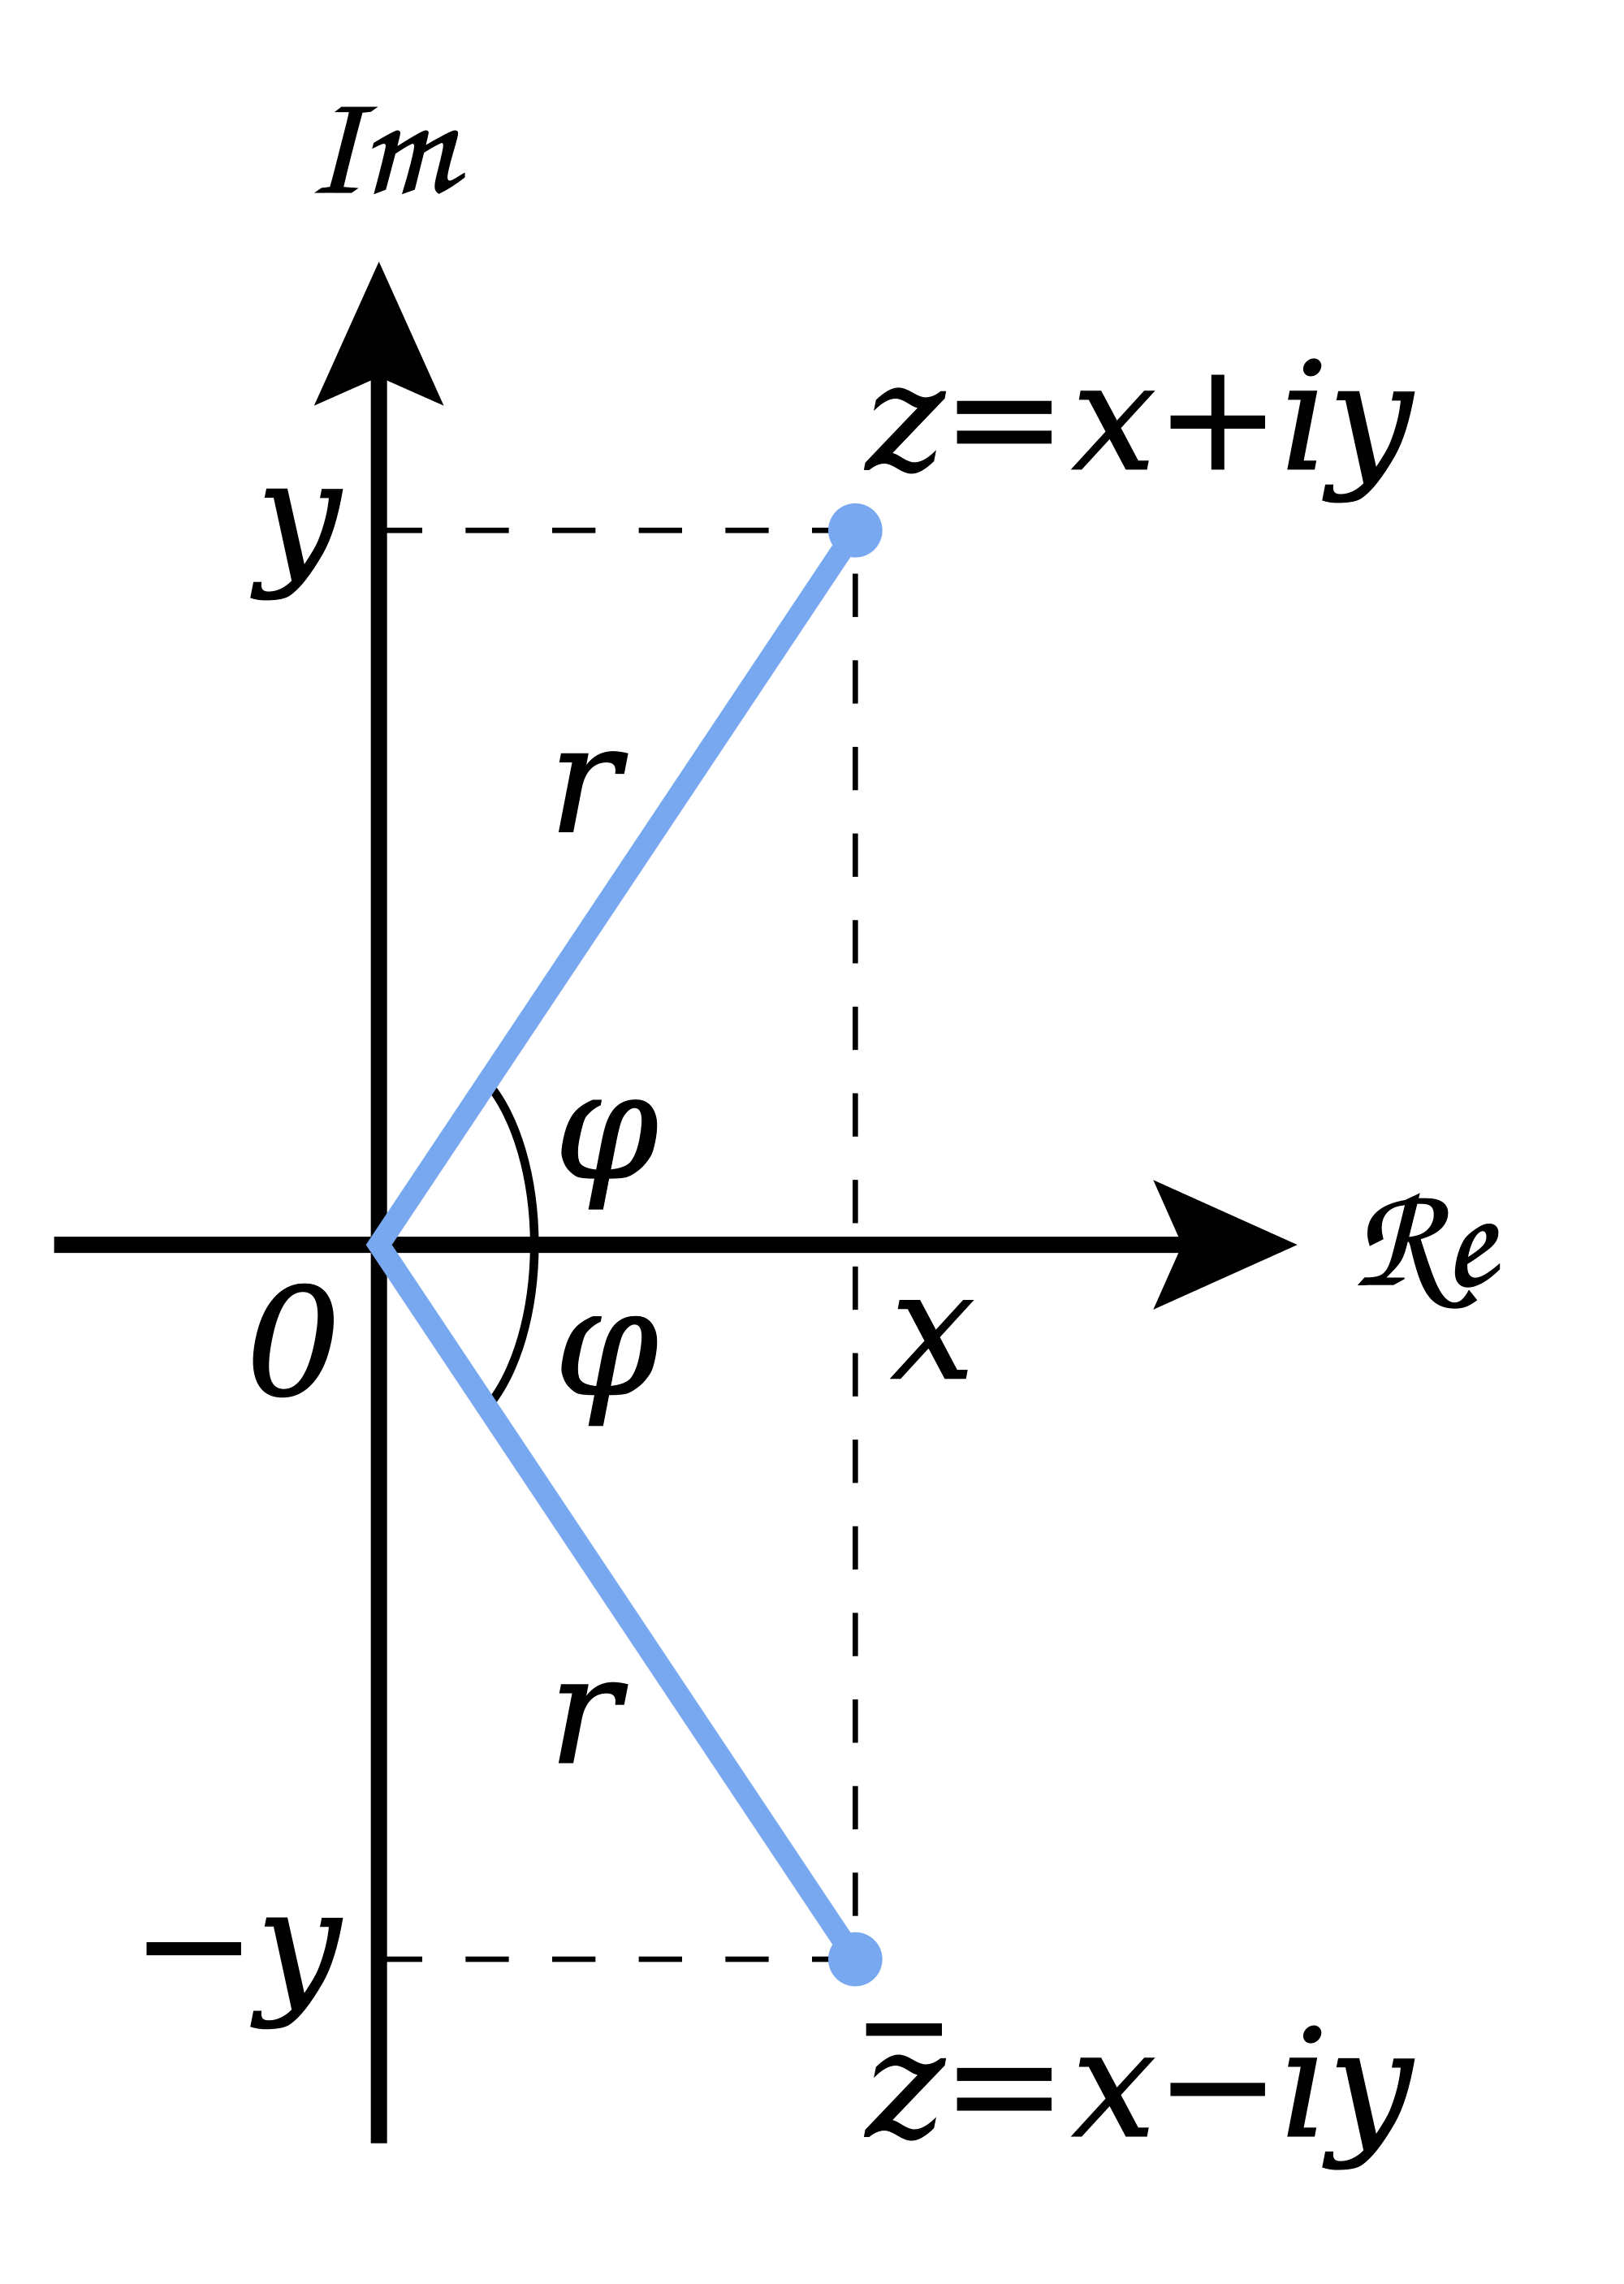
\includegraphics[scale=0.05]{wessel-plane.png}
	\caption{Wessel Plane Plot: (Complex conjugate picture.svg from Wikimedia Commons)}
\end{figure}
\section{Linear Vector Spaces} 
A linear vector space or simply a vector space $\mathbb{V}$ is a set along with the regular multiplication and addition operations over a field $\mathcal{F}$, such that the following axioms hold: \footnote{Here, $\alpha , \beta \in \mathcal{F}$ and $\mathcal{U}, \mathcal{V} $ and $\mathcal{W} \in \mathbb{V}$} \\
\subsection{Commutativity}
$$\mathcal{U} + \mathcal{V} = \mathcal{V} + \mathcal{U}$$
\subsection{Associativity}
$$(\mathcal{U} + \mathcal{V}) + \mathcal{W} = \mathcal{V} + (\mathcal{U} + \mathcal{W})$$
$$(\alpha \beta) \mathcal{V} = \alpha (\beta \mathcal{V})$$
\subsection{Additive Identity}
$$\exists \  0 \in \mathbb{V} \ | \ \mathcal{V} + 0 = 0 + \mathcal{V} = \mathcal{V}$$
\subsection{Additive Inverse}
$$\forall \ \mathcal{V} \ \exists \ \mathcal{V}^{-1} \ | \ \mathcal{V} + \mathcal{V} = 0$$
\subsection{Multiplicative identity}
$$\exists \ 1 \in \mathbb{V} \ | \ 1 \mathcal{V} = \mathcal{V}$$
\subsection{Distributive properties}
$$\alpha (\mathcal{U} + \mathcal{V}) = \alpha \mathcal{U} + \alpha \mathcal{V}$$
$$(\alpha + \beta) \mathcal{U} = \alpha \mathcal{U} + \beta \mathcal{U}$$
\section{Inner Product Spaces}
An inner product is simply an operation that takes a Dual $\ket{\psi}$ and it's corresponding vector $\bra{\psi}$ and maps them to $\mathbb{R}$:
$$\braket{expression1}{expression2}$$
\section{Dual Spaces}
\section{Dirac Notation}
Operators are represented with respect to a particular basis (in this case $\{e_{m}, e_{n}\}$) by their matrix elements
\begin{equation}
\langle e_{m}| \hat{O} | {e_n} \rangle = \hat{O}_{mn}
\end{equation}
\section{Subspaces}
Given a vector space $\mathbb{V}$, a subset of its elements that form a vector space among themselves is called a subspace. We will denote a particular subspace $i$ of dimensionality $n_{i}$ by $\mathbb{V}^{n_{i}}_{i}$.\\
   Given two subspaces, and , we define their sum $\mathbb{V}^{n_{i}}_{i} \oplus \mathbb{V}^{m_{i}}_{i} = \mathbb{V}^{l_{i}}_{i}$ \footnote{Here $\oplus$ is the direct sum defined as: } as the set containing:
\begin{enumerate}
\item All the elements of $\mathbb{V}^{n_{i}}_{i}$
\item All the elements of $\mathbb{V}^{m_{j}}_{j}$
\item And all possible linear combinations of the above
\end{enumerate} 
However for the elements of (3), closure is lost. The dimensionality of such a subspace is $n + m$.
\section{Hilbert Spaces}
A Hilbert space $H$ is simply a normed vector space (a Banach space), whose norm is defined as:
\begin{equation} \label{norm}
\norm{V} := \sqrt{\braket{V}{V}}
\end{equation}
This is an axiomatic definition of a Hilbert space, but we are more concerned with the corollaries of it. All the Cauchy sequences \footnote{Defintion} of functions in a Hilbert space always converge to a function that is also a memeber of the space i.e. it is said to be \textbf{complete} which implies that the integral of the absolute square of a function must converege \footnote{we simply state this but a proof can be found in}
\begin{equation}
\int_{a}^{b} \abs{f(x)}^{2} dx < \infty
\end{equation}
Moreover this means that, any function in Hilbert space can eb expressed as a linear combination of other functions i.e. it is closed/complete
\begin{equation}
f(x) = \sum_{n = 1}^{\infty} c_{n} f_{n}(x)
\end{equation}
Where, $c_{n} \in \mathbb{C}$
\section{Linear Operators}
\section{Eigenvalue Problem}
\section{Eigenfunctions of a Hermitian Operator}

\section{Transformations}
\subsection{Active Tranformation}
In a loose sense this can be thought of as,

\subsection{Passive Tranformation}
From our discussion before it is also clear that the same transformation can be implemented as,
\begin{equation}
\hat{O} \rightarrow U^{\dagger}\hat{O}U
\end{equation}
This is a very different viewpoint, we can understand this by visualizing it to be a 
\subsection{Equivalence of Transformation types}
It's pretty simple to see that both types of transformation constitute the same physical picture. Thus, we can take both viewpoints to mean the same physical transformation in each case, and later on we will see how this leads us two different pictures of Quantum Mechanics and how they are related.
\section{Functions of Operators}
\section{Generalization to Infinite Dimensions}
\section{Probability}
\subsection{Discrete Variables}
Suppose we have a frequency distribution 
\begin{equation}
N = \sum_{j=0}^{\infty} N(j)
\end{equation}
The probability of an event $N_{j}$ is defined as,
\begin{equation}
P(j) = \frac{N(j)}{N}
\end{equation}
In probability theory, the sum of all probabilities is 1,
\begin{equation}
\sum_{j = 0}^{\infty}P(j) = \sum_{j = 0}^{\infty}\frac{N(j)}{N} = 1
\end{equation}
The average/mean/expectation value of a value $j$ is given by the formula:
\begin{equation}
	\expval{j} = \frac{\sum j N(j)}{N} = \sum_{j =0 }^{\infty} j P(j)
\end{equation}
and in general, the average of some function of $j$, is given by,
\begin{equation}
\expval{f(j)} = \sum_{j =0 }^{\infty} f(j) P(j)
\end{equation}
The spread of a variable's value from it's mean is called it's variance, written as
\begin{equation}
\sigma^{2} = \expval{{(\Delta j)}^{2}}
\end{equation}
where,
$$\Delta j = j - \expval{j}$$
It's square root is called the standard deviation,
\begin{equation}
\sigma = \sqrt{\expval{{(\Delta j)}^{2}}} =  \sqrt{\expval{j^{2}} - \expval{j}^{2}}
\end{equation}
Which comes from a theorem on variances that we'll find useful later on:
$$\sigma^{2} = \expval{{(\Delta j)}^{2}} = \sum {(\Delta j)}^{2} P(j) = \sum {(j- \expval{j})}^{2} P(j)$$
$$ = \sum (j^{2} - 2j \expval{j} + \expval{j}^{2}) P(j)$$
$$ = \sum j^{2}P(j) - 2 \expval{j} \sum jP(j) + \expval{j}^{2}\sum P(j)$$
$$ = \expval{j^{2}} - 2 \expval{j}\expval{j} + \expval{j}^{2} = \expval{j^{2}} - \expval{j}^{2}$$
\subsection{Continuous Variables}
We now move to a continuous probability distribution, we'll create continuous analogs of all the quantities we just introduced. Let's start with probability, the probability of that $x$ lies between $a$ and $b$
\begin{equation}
	P_{ab} = \int_{a}^{b} \rho(x) dx
\end{equation}
where $\rho(x)$ is the called the probability density i.e. the probability of getting $x$, or more concretely,
$$\rho(x)dx = \text{Probability that an individual is chosend at random lies between } x \text{ and } x + dx$$
Now supposing the rules we held for discrete variables hold, the continuous analogs look like this:
\begin{equation}
	1 = \int_{- \infty}^{\infty} \rho(x) dx
\end{equation}
\begin{equation}
	\expval{x} = \int_{- \infty}^{\infty} x \rho(x) dx
\end{equation}
\begin{equation}
	\expval{f(x)} = \int_{- \infty}^{\infty} f(x) \rho(x) dx
\end{equation}
\begin{equation}
	\sigma^{2} := \expval{(\Delta x)^{2}} = \expval{x^{2}} - {\expval{x}}^{2}
\end{equation}
\section{Expectation Values}
In this section we'll explore how we express the expectation values of a few opeartors. Let's start with the position opeartor in the position representation (i.e. position basis):
\begin{equation} \label{posex}
	\expval{x} = \int_{- \infty}^{\infty} x \abs{\psi(\vec{x}, t)}^{2} dx
\end{equation}
We can differentiate \ref{posex} with respect to time to find the expectation value for "velocity":
$$\frac{d \expval{x}}{dt} = $$
Throwing away 
\begin{equation}
	\expval{v} = \frac{d \expval{x}}{dt} = -\frac{i \hbar}{m} \int \psi^{*} \frac{\partial \psi}{\partial x} dx
\end{equation}
Therefore we can write the expectation value of momentum as,
\begin{equation}
	\expval{p} = m \frac{d \expval{x}}{dt} =  -i \hbar \int \left(\psi^{*} \frac{\partial \psi}{\partial x} \right) dx
\end{equation}
In general, every observable is a function of position and momentum, thus for an observable $\hat{O}(x,p)$, the expectation value is given by,
\begin{equation}
	\expval{\hat{O}(x,p)} = \int \psi^{*} \hat{O}(x,-i \hbar \nabla) \psi dx
\end{equation}
For example, the expectation value of kinetic energy is,
\begin{equation}
\expval{T} = -\frac{\hbar^{2}}{2m} \int \psi^{*} \frac{\partial^{2} \psi}{\partial x^{2}} dx
\end{equation}
Or to sum it up in Dirac notation,
\begin{equation}
	\expval{\hat{O}} = \expval{\hat{O}}{\psi}
\end{equation}
\section{Fourier Analysis}
\subsection{Dirichelet's Theorem}

\subsection{Fourier Transform}

\section{Delta Function}
\subsection{The Divergence of $\frac{\hat{r}}{r^{2}}$}
We can see why the divergence is,
\begin{equation}
\nabla . \frac{\hat{r}}{r^{2}} = 0
\end{equation}
But if we calculate this using the Divergence theorem, we find that ,
\begin{equation}
	\oint v .da = \int \left( \frac{\hat{r}}{r^{2}} \right) . \left( r^{2} \sin(\theta) d \theta d \phi \hat{r} \right) = \left( \int_{0}^{\pi} \sin(\theta) d \theta \right) \left( \int_{0}^{2\pi} d \phi \right) = 4 \pi
\end{equation}
This is paradoxical. The issue is that it blows up at $r=0$ but is is neglible everywhere else. How do we fix this? The Dirac Delta functional!
\subsection{The One-Dimensional Dirac Delta Functional}
The Dirac Delta is a functional \footnote{An object that is a map between functions} which we define as,
\begin{equation} \label{deltadef}
\delta(x-a)= 
\begin{cases}
0, & \text{if } x \neq a\\
\infty,              & \text{if } x = a
\end{cases}
\end{equation}
\begin{equation}
\int_{- \infty}^{+ \infty} \delta(x-a) dx = 1
\label{del2}
\end{equation}
$\forall \  a \in \mathbb{R}$
We can visualize it as a sharp peak at $a$,
\begin{figure}
	\centering
	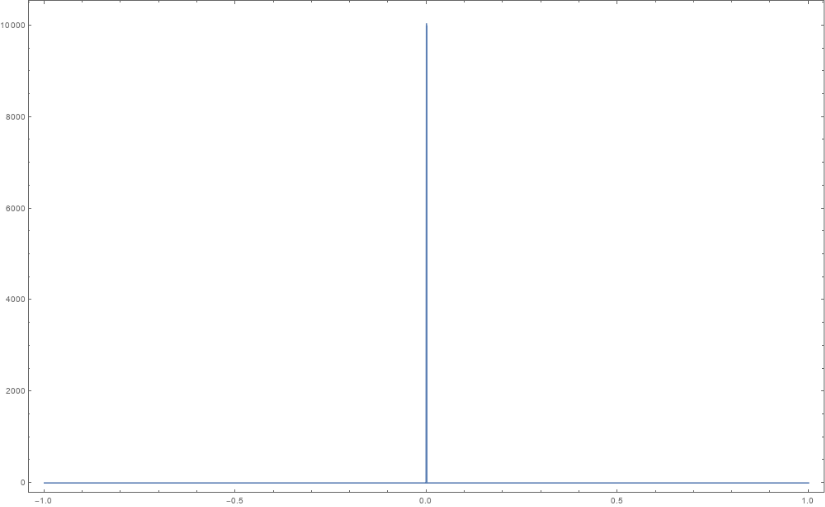
\includegraphics[scale=0.5]{delta-distribution.png}
	\caption{A Plot of $\delta(x)$}
\end{figure}
We can interpret \ref{del2} as saying "the area of the delta distribution is always 1".
\begin{equation}
f(x)\delta(x - a ) = f(a)
\end{equation}
We can combine these to get,
\begin{equation}
\int_{- \infty}^{+ \infty} \delta(x-a) f(x) dx = f(a)
\end{equation}
\subsubsection{A few interesting properties}
\begin{equation}
\delta(kx) = \frac{1}{|k|}\delta(x)
\end{equation}
\begin{equation}
\frac{d}{dx}(\delta(x)) = -\delta(x)
\end{equation}
where k is a constant
\begin{equation}
\frac{d \theta}{dx} = \delta(x)
\end{equation}
Where $\theta$ is the step function defined as,
\begin{equation}
\theta(x)= 
\begin{cases}
1, & \text{if } x > 0\\
o,              & \text{if } x \leq 0
\end{cases}
\end{equation}

\subsection{The Three-Dimensional Dirac Delta Function}
We generalize (\ref{deltadef}) to three dimensions,
\begin{equation}
\delta^{3}(\vec{r} - \vec{a}) = \delta(x-a_{x})\delta(y-a_{y})\delta(z-a_{z})
\end{equation}
\begin{equation}
\int_{- \infty}^{+ \infty} \delta^{3}(\vec{r} - \vec{a}) dV = 1
\end{equation}
We can also define the three-dimensional delta function as
\begin{equation}
\delta^{3}(\boldscriptr) = \frac{1}{4 \pi} \left[\nabla \cdot \left( \frac{\hat{\boldscriptr}}{{\scriptr	}^{2}}\right)\right]
\end{equation}
Since,
$$\nabla \left(\frac{1}{\scriptr}\right) = -\frac{\hat{\boldscriptr}}{\scriptr^{2}}$$
We can rewrite as,
\begin{equation}
\delta^{3}(\boldscriptr) = -\frac{1}{4 \pi} \left[\nabla^{2}  \left( \frac{1}{\scriptr}\right)\right]
\end{equation}
\section{Gaussian Integrals}
\section{The $i \epsilon$ Prescription}
We will now derive and interpret the formula:
\begin{equation}
\frac{1}{x \mp i \epsilon} = \mathscr{P} \frac{1}{x} \pm \pi \delta (x)
\end{equation}
where $\epsilon \rightarrow 0$ is a positive infinitesimally small quantity. Now we'll consider the integral
\begin{equation}
	content...
\end{equation}
$$$$
\begin{equation}
a
\end{equation}
\begin{equation}
asdfkjh
\end{equation}
\section{Permutation Functions}
\subsection{Kronecker delta}
It simply has the ‘function’ of ‘renaming’ an index:
$$\delta^{\mu}_{\nu} x^{\nu} = x^{\mu}$$
it is in a sense simply the identity matrix. Or it is sometimes defined as:
\begin{equation}
\delta_{ij} = \begin{cases}
1 \ \text{if } i = j \\
0 \ \text{if } i \neq j\\
\end{cases}
\end{equation}
\subsection{Levi-Civita Pseudotensor}
\label{Levi}
The Levi-Civita Pseudotensor i.e. Tensor density is a completely anti-symmetric i.e. $\epsilon_{ijk} = -\epsilon_{jik} = -\epsilon_{ikj} = -\epsilon_{kji}$, we define it as:
\begin{equation}
\epsilon_{ijk} = \begin{cases}
1 \ \text{if } ijk \text{ is an even permuation of } 123\\
-1 \ \text{if } ijk \text{ is an odd permuation of } 123\\
0  \text{ if two indices are equal}\\
\end{cases}
\end{equation}
\subsubsection{Identities}
\begin{equation}
\epsilon_{\alpha \beta \nu}\epsilon_{\alpha \beta \sigma} = \delta_{\mu \rho} \delta_{\nu \sigma} - \delta_{\mu \sigma}\delta_{\nu \rho}
\end{equation}
From this it follows that,
\begin{equation}
\epsilon_{\alpha \beta \nu}\epsilon_{\alpha \beta \sigma} = 2\delta_{\nu \sigma}
\end{equation}
and
\begin{equation}
\epsilon_{\alpha \beta \gamma}\epsilon_{\alpha \beta \gamma} = 6
\end{equation}
\section{Tensors}
\section{Variational Calculus}